% chktex-file 8

\chapter{Amazon EMR Tutorial}

Scott Steinbruegge, hid-sp18-521

\section{Introduction}

Amazon EMR is a Hadoop framework that allows users to process data on the AWS 
platform using their EC2 technology to spread the load across multiple EC2 
instances. Elasticity a major benefit of EMR as it can be set to auto scale 
up or down the number of EC2 instances that EMR is running in a cluster. The 
user can choose to run additional frameworks supported on EMR in addition 
to Hadoop, such as Spark, HBase, Flink and Presto. The platform allows the 
user to focus on the processing of the data and not have to deal with the 
setup, management or tuning of a Hadoop cluster. Using EMR allows a user 
to setup and provision a cluster quickly and allows for scalability of 
compute resources up or down and in or out as needed. Interactions with 
EMR can occur through a web service interface or by using the AWS 
Management Console to launch and monitor clusters. In this tutorial, 
setup and configuration of an EMR cluster will be done through the AWS 
Management Console. 

\section{Prerequisites}

Before proceeding with any steps to create an EMR cluster, you need to 
ensure that you have an AWS account setup. If not, you need to have one 
created before continuing with this tutorial. Afterwards, sign into the 
AWS Management Console. There are two prerequisites that need to be met 
before being able to launch an EMR cluster, setup an S3 bucket and an EC2 
key pair. The S3 bucket you create will be used for storing the EMR logs 
and any output data produced by your EMR cluster. Bucket names have several 
constraints that need to be met due to Hadoop requirements such as only 
consisting of lowercase letters, numbers, periods, hyphens and also cannot 
end in numbers~\cite{hid-sp18-521-prereq}. In order to create the S3 bucket, 
go to S3 section of the AWS Management Console and select the `Create bucket' 
button. Fill in the requested information for bucket name and region, then 
proceed to the next two pages to enter in the bucket properties and 
permissions. After those sections, a review page will be presented for your 
review and if you are satisfied with your selections, 
click `Create bucket`~\cite{hid-sp18-521-s3bucket}. 

\begin{center}
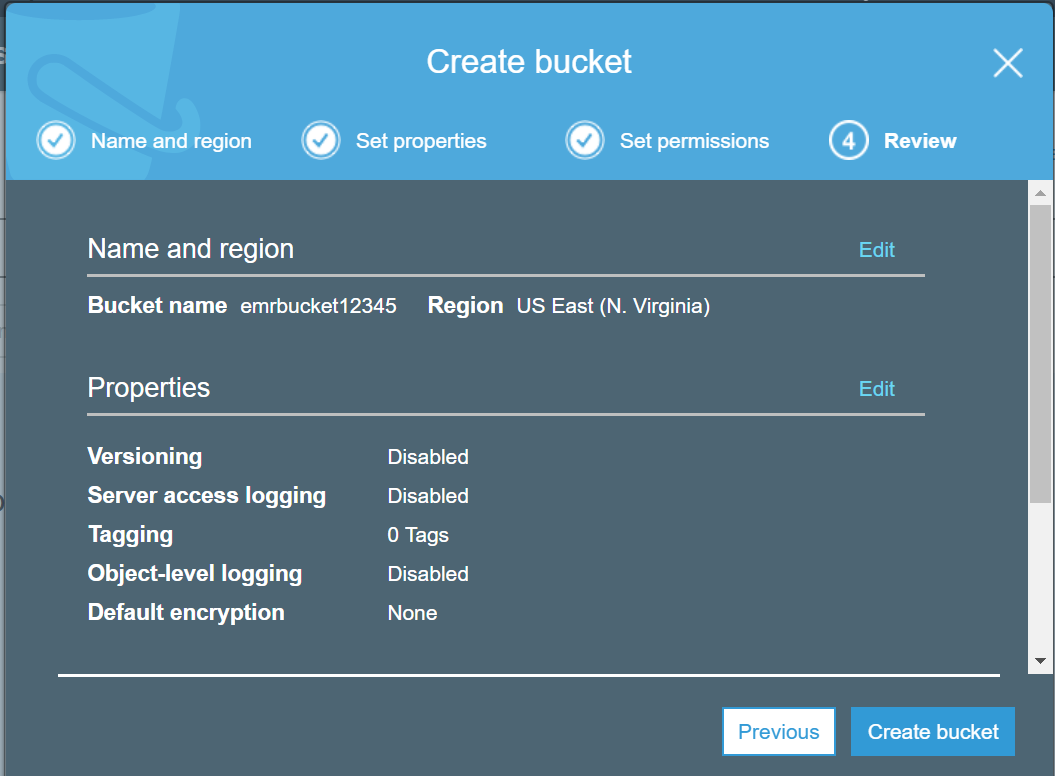
\includegraphics[width=\columnwidth]{images/S3_create_bucket.png}
\end{center}

After the S3 bucket has been created, an EC2 key pair then needs to be 
generated which allows you to connect to your EMR cluster over SSH\@. If you 
already have an existing EC2 key pair that can be used for this tutorial as 
well. In order to generate an EC2 key pair through the AWS Management Console, 
search and navigate to the EC2 section from the console home page. In the pane 
on the left side of the screen, look for the `Network and Security' section 
and select the `Key Pairs' option. On the next page select `Create Key Pair' 
button and type in a name you want to give this key pair.  After you select 
the key name click `Create' and your EC2 key pair wil be automatically 
downloaded by the browser and named with a pem extension. Save the key file 
generated in a safe location for use later on as this is the only time you will 
be able to save this key file. It will need to be used when you need to launch 
and connect to the EC2 instances created by EMR~\cite{hid-sp18-521-ec2keypair}. 

\begin{center}
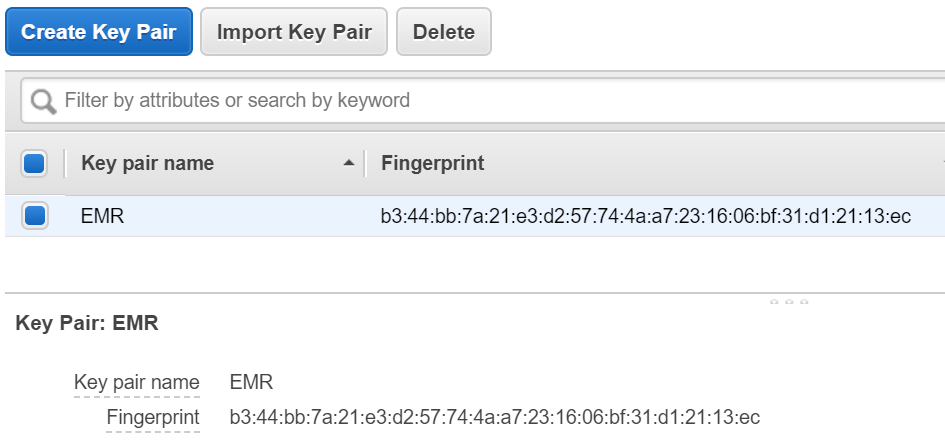
\includegraphics[width=\columnwidth]{images/EMRkey.png}
\end{center}

\section{Configuring and Utilizing the Cluster with AWS Management Console}

Once all the prerequisites above have been met, an EMR cluster can now be 
created. In the AWS Management Console home page, enter in `EMR' in the AWS 
services search box at the top of the page and select the EMR option that it 
returns. You will be taken to the EMR home page. At the top of this page is 
a button labeled `Create cluster'. Click this button and you will be brought 
to the screen where you can select cluster creation options. By default, it 
brings up the quick options page which allows you to select basic options 
needed to setup and configure an EMR cluster. There is also an option to show 
advanced options that can be used for cluster creation at the top of the page. 
Stay on the quick options page for now and enter in the cluster name, which is 
optional. You then select if you would like to enable logging. If so, you can then 
select a location in S3 where you would like the logs to be placed. There are then 
two options to choose from for launch mode: cluster or step execution. The 
cluster option can be used for EMR clusters that you want to remain online 
indefinitely. The step execution option would be used for when you want to 
execute a set of predefined steps upon cluster creation and once those steps 
complete successfully, shut down the cluster~\cite{hid-sp18-521-emrlaunch}. 

\begin{center}
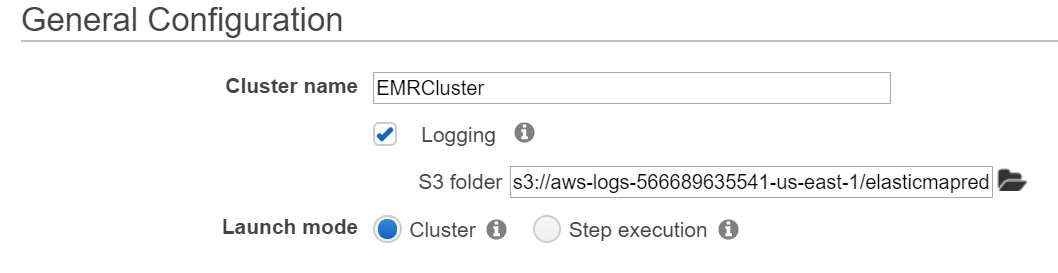
\includegraphics[width=\columnwidth]{images/emr_gen_config.png}
\end{center}

Once launch mode is selected, scroll down to the `Software configuration' 
section and choose an EMR release version. The most current version is 
selected by default. If you chose a cluster launch mode, then proceed to 
selecting one of the 4 predefined sets of applications you want to install 
based on your use case. If step execution was selected instead of cluster, 
then the core Hadoop install is the only application option you can use 
here. Now move on to the `Hardware configuration' and select the EC2 instance 
type and number of EC2 instances you would like to utilize for your cluster. 
he values selected here will vary on what type of data processing you`re 
looking to achieve. Then scroll down to the `Security and access' section 
of the page and select the key pair generated in the steps above in the 
drop-down menu. Below that you can then select which permissions model to u
se: default or custom. The default option sets up permissions for your EMR 
cluster that are granted using policies applied to EMR specific IAM roles. 
Using the custom option allows you to select existing IAM roles to apply 
permissions to instead of creating new roles. Once all of this information 
has been selected, the cluster is then ready to be launched by selecting 
the `Create cluster' button at the bottom of the page. Your cluster will 
then be launched and ready for workloads~\cite{hid-sp18-521-emrlaunch}. 

\begin{center}
\centering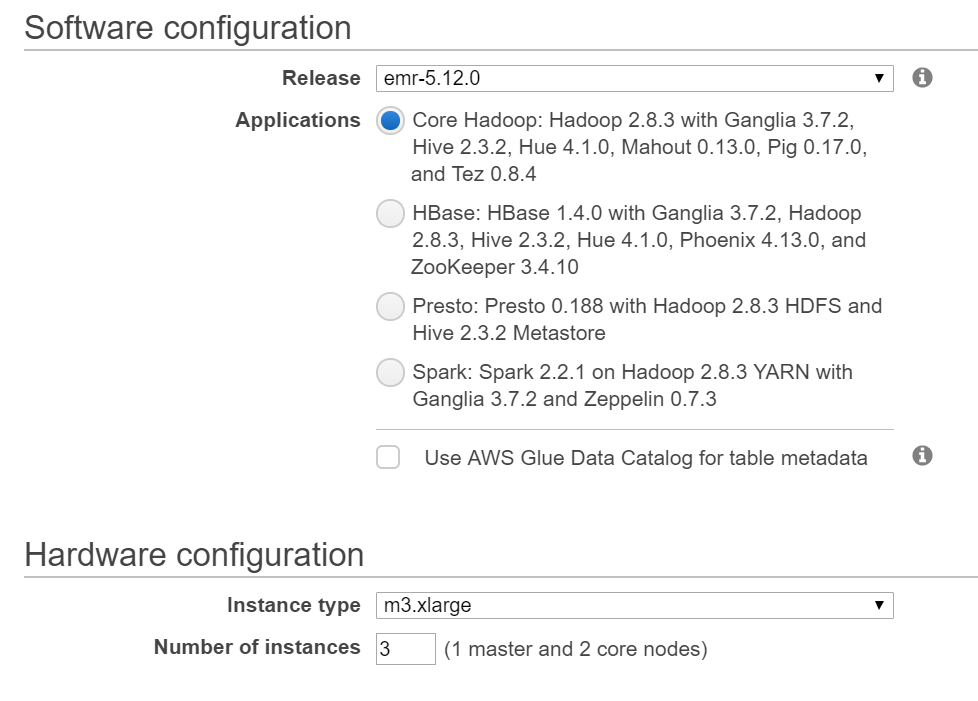
\includegraphics[width=\columnwidth]{images/emr_software_config.png}

\centering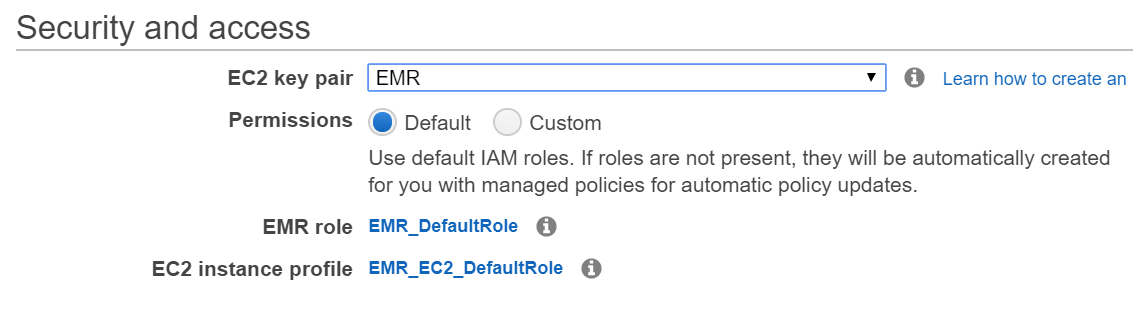
\includegraphics[width=\columnwidth]{images/emr_security.png}
\end{center}

If you`ve selected cluster launch mode, ad-hoc processing of data can now 
occur on cluster. To get started go to the EMR console page. From here you can 
then select the `Clusters' menu on the left side of the screen which will 
then show you a list of current EMR clusters you have setup. Click on the 
name of the cluster you would like to run processing steps on and then navigate 
over to the `Steps' tab on the following page. You show see a button named 
`Add step' which you can then select to setup the type of step you would like to 
run for data processing. The step types available to create vary based on the 
applications that were installed during the creation of the cluster. In this 
example, only the core Hadoop applications were installed, so the step types 
are limited to custom JAR, Hive, Pig and streaming programs. Each step type 
then has a set of parameters that need to be populated before the step can be 
created. After you`ve decided on a step type and have populated all of the 
required step parameters, click the `Add' button which will then create and 
run the step on the cluster. This process can be repeated as needed and there 
are additional ways to submit up to 256 active steps that can be explored but 
is beyond the scope of this tutorial~\cite{hid-sp18-521-emrprocess}.  

\begin{center}
\centering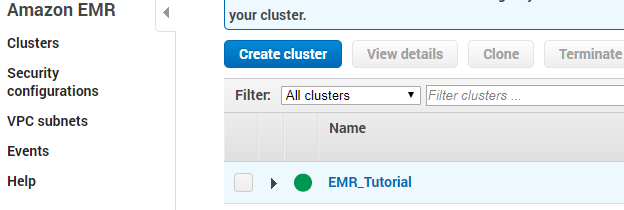
\includegraphics[width=\columnwidth]{images/emr_cluster_create.png}

\centering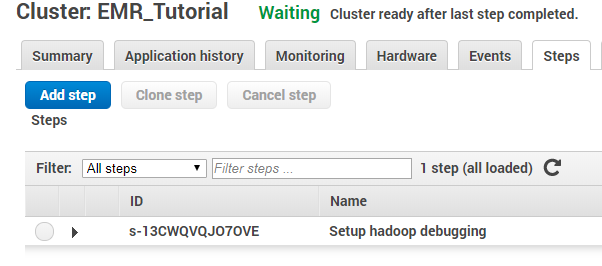
\includegraphics[width=\columnwidth]{images/emr_cluster_steps.png}

\centering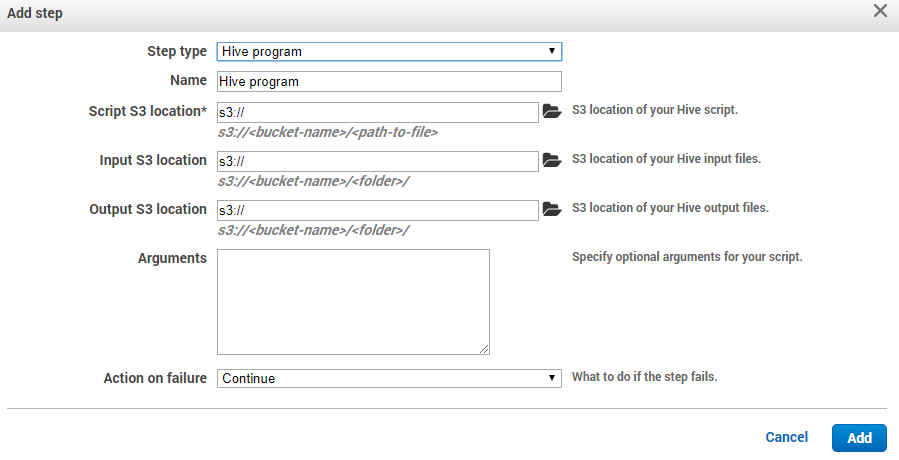
\includegraphics[width=\columnwidth]{images/emr_cluster_steps2.png}
\end{center}

\section{Teardown}

Once completing the steps in the tutorial, it is recommended that you cleanup 
what you`ve created in order to avoid high costs of usage. The S3 bucket you 
created along with the EMR cluster itself will need to be removed. Start with 
the termination of the cluster by going to main EMR page and selecting the 
`Cluster' option on the left. Select the check box for the name of the cluster 
you wish to terminate and click the `Terminate' button. It will them prompt 
you to confirm this clusters termination which you will verify and continue. 
This will place the cluster in a `Terminating' state and eventually move to 
a `Terminated' state. Terminated clusters will remain viewable in the console 
for two months. You can then proceed to the S3 console page. Before you can 
delete buckets, you have to delete all of the folders and files contained 
within that bucket. To do this, click on the bucket name which will then show 
the subfolders contained within the bucket. Check the box next to all of the 
subfolder names, select the `More' button in the menu above and from that 
menu select `Delete'. Once all of the folders and files are gone, navigate 
back to the main S3 page, click the row of the bucket name you wish to delete 
and select the `Delete' button. You will then be prompted to enter the name 
of the bucket you wish to delete and select the `Confirm' button before the 
deletion occurs. Once your EMR cluster has been successfully terminated and 
all buckets created during the tutorial have been deleted, you can then be 
certain that no additional costs will continue to accrue based on the work 
performed in this tutorial~\cite{hid-sp18-521-emrreset}.  

\begin{center}
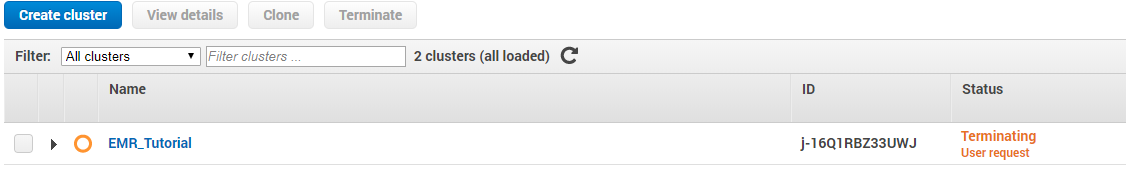
\includegraphics[width=\columnwidth]{images/emr_terminate.png}

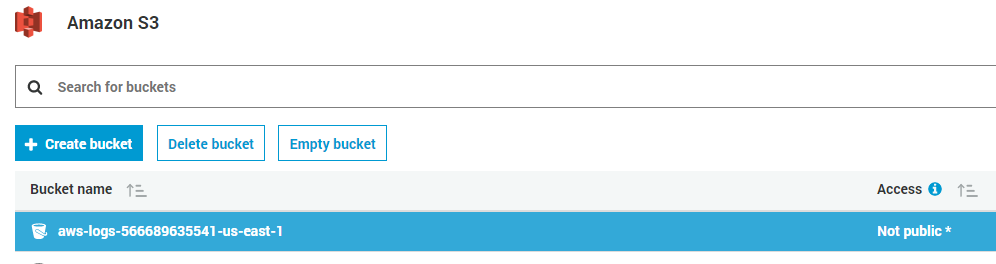
\includegraphics[width=\columnwidth]{images/s3_delete_bucket.png}
\end{center}
